%%%%%%%%%%%%%%%%%%%%%%%%%%%%%%%%%%%%%%%%%
% Beamer Presentation
% LaTeX Template
% Version 1.0 (10/11/12)
%
% This template has been downloaded from:
% http://www.LaTeXTemplates.com
%
% License:
% CC BY-NC-SA 3.0 (http://creativecommons.org/licenses/by-nc-sa/3.0/)
%
%%%%%%%%%%%%%%%%%%%%%%%%%%%%%%%%%%%%%%%%%

%----------------------------------------------------------------------------------------
%	PACKAGES AND THEMES
%----------------------------------------------------------------------------------------

\documentclass{beamer}

\mode<presentation> {

% The Beamer class comes with a number of default slide themes
% which change the colors and layouts of slides. Below this is a list
% of all the themes, uncomment each in turn to see what they look like.

%\usetheme{default}
%\usetheme{AnnArbor}
%\usetheme{Antibes}
%\usetheme{Bergen}
%\usetheme{Berkeley}
%\usetheme{Berlin}
%\usetheme{Boadilla}
%\usetheme{CambridgeUS}
\usetheme{Copenhagen}
%\usetheme{Darmstadt}
%\usetheme{Dresden}
%\usetheme{Frankfurt}
%\usetheme{Goettingen}
%\usetheme{Hannover}
%\usetheme{Ilmenau}
%\usetheme{JuanLesPins}
%\usetheme{Luebeck}
%\usetheme{Madrid}
%\usetheme{Malmoe}
%\usetheme{Marburg}
%\usetheme{Montpellier}
%\usetheme{PaloAlto}
%\usetheme{Pittsburgh}
%\usetheme{Rochester}
%\usetheme{Singapore}
%\usetheme{Szeged}
%\usetheme{Warsaw}

% As well as themes, the Beamer class has a number of color themes
% for any slide theme. Uncomment each of these in turn to see how it
% changes the colors of your current slide theme.

%\usecolortheme{albatross}
%\usecolortheme{beaver}
%\usecolortheme{beetle}
%\usecolortheme{crane}
%\usecolortheme{dolphin}
%\usecolortheme{dove}
%\usecolortheme{fly}
%\usecolortheme{lily}
%\usecolortheme{orchid}
%\usecolortheme{rose}
%\usecolortheme{seagull}
%\usecolortheme{seahorse}
%\usecolortheme{whale}
%\usecolortheme{wolverine}

%\setbeamertemplate{footline} % To remove the footer line in all slides uncomment this line
%\setbeamertemplate{footline}[page number] % To replace the footer line in all slides with a simple slide count uncomment this line

%\setbeamertemplate{navigation symbols}{} % To remove the navigation symbols from the bottom of all slides uncomment this line
}

\usepackage{graphicx} % Allows including images
\usepackage{booktabs} % Allows the use of \toprule, \midrule and \bottomrule in tables
\usepackage{tikz}
\usepackage[utf8]{inputenc} 
\usepackage{amsmath,tkz-base} 
\usetikzlibrary{matrix, fit,calc,positioning,decorations.pathreplacing}
\usepackage{pstricks}
\usepackage{pst-plot}
\setbeamerfont{block body}{size=\small}
\usepackage{gensymb}

\psset{xunit=.01cm, yunit = 1cm}
% Create command that makes margin wider for one slide
% ------------------------------------------------------------
\newcommand\Wider[2][3em]{%
\makebox[\linewidth][c]{%
  \begin{minipage}{\dimexpr\textwidth+#1\relax}
  \raggedright#2
  \end{minipage}%
  }%
}
% ------------------------------------------------------------


%----------------------------------------------------------------------------------------
%	TITLE PAGE
%----------------------------------------------------------------------------------------

\title[In silico pathogens]{In silico prediction: pathogens in synthetic communities} % The short title appears at the bottom of every slide, the full title is only on the title page

\author{Wai Kit Tsang} % Your name

\institute[LabMET \& Kermit] % Your institution as it will appear on the bottom of every slide, may be shorthand to save space
{
Promotors: Prof. dr. ir. Nico Boon \&  \\ Prof. dr. Willem Waegeman \\ tutor: dr. Ramiro V\'ilchez Vargas \& ir. Michiel Stock \\
\medskip
Ghent University \\ % Your institution for the title page
\medskip
\textit{waikit.tsang@ugent.be} % Your email address
}
\date{\today} % Date, can be changed to a custom date

\begin{document}

\begin{frame}
\titlepage % Print the title page as the first slide
\end{frame}

\begin{frame}
\frametitle{Overview} % Table of contents slide, comment this block out to remove it
\tableofcontents % Throughout your presentation, if you choose to use \section{} and \subsection{} commands, these will automatically be printed on this slide as an overview of your presentation
\end{frame}

%----------------------------------------------------------------------------------------
%	PRESENTATION SLIDES
%----------------------------------------------------------------------------------------

%------------------------------------------------
\section{Introduction} % Sections can be created in order to organize your presentation into discrete blocks, all sections and subsections are automatically printed in the table of contents as an overview of the talk
%------------------------------------------------

%\subsection{Wet Lab Experiments vs In silico Prediction} % A subsection can be created just before a set of slides with a common theme to further break down your presentation into chunks

\begin{frame}
\frametitle{Predictive modelling}
\begin{columns}[c] % The "c" option specifies centered vertical alignment while the "t" option is used for top vertical alignment

\column{.45\textwidth} % Left column and width
\textbf{Motivation}
\begin{itemize}
\item Interest: predictive modelling
\item Gathering the data
 
\end{itemize}

\column{.5\textwidth} % Right column and width
Combining Wet Lab Experiments with In silico prediction.
\end{columns}

\end{frame}

%------------------------------------------------

\begin{frame}
\frametitle{Microbial Relevance}
\begin{columns}[c] % The "c" option specifies centered vertical alignment while the "t" option is used for top vertical alignment

\column{.45\textwidth} % Left column and width
\textbf{Microbial Ecology}
\begin{itemize}
\item Pathogen Behaviour after invasion
\item Does evenness play a role?
 
\end{itemize}

\column{.5\textwidth} % Right column and width
\textbf{Predictive Modelling}
\begin{itemize}
\item Quite Robust Against varying data
\item Cover enough points in the feature space
 
\end{itemize}
\end{columns}
\end{frame}

%------------------------------------------------

%------------------------------------------------
\section{Research Question}
%------------------------------------------------

\begin{frame}
\frametitle{Concept of evenness}
Relative abundance of species in a community.
\newline

\begin{tikzpicture}[scale = .8]
\tkzInit[xmax=1,ymax=350,xstep=.1,ystep=50]
\tkzAxeX[label=$x$]
    \node[anchor=center] at (5, -1.1) {Pielou's Evenness};
    \node[anchor=center] at (0, -1) {Low};
    \node[anchor=center] at (10, -1) {High};
    % Include the figures
    \node[inner sep=0pt] (low_evenness) at (0,2)
    	{ 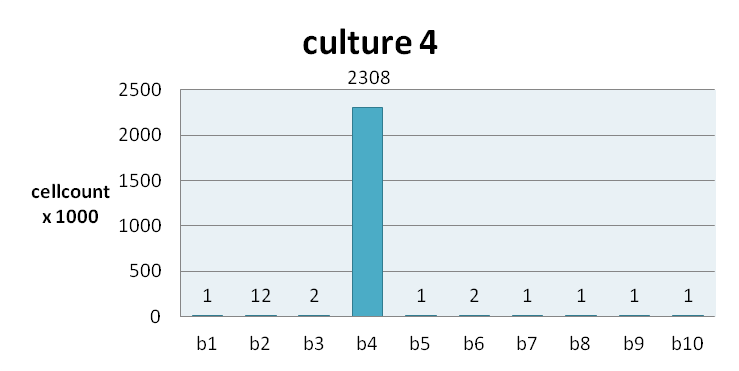
\includegraphics[scale = .3, trim = 5 5 5 5, clip]{c4.png} };
    \node[inner sep = 0 pt] (mid_evenness) at(4.5, 2)
    	{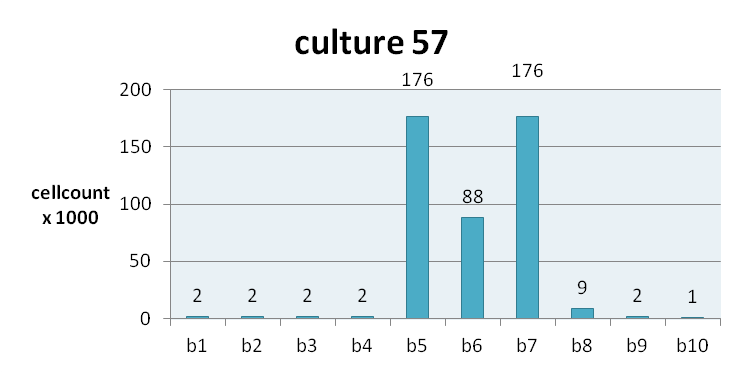
\includegraphics[scale = .3, trim = 5 5 5 5, clip]{c57.png}};
    \node[inner sep = 0 pt] (high_evenness) at(9, 2)
       	{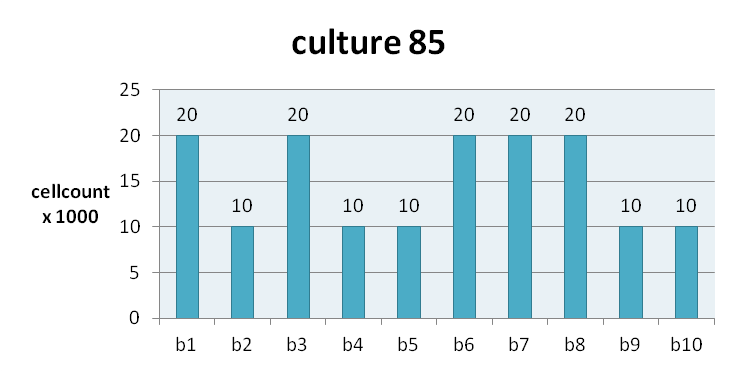
\includegraphics[scale = .3, trim = 5 5 5 5, clip]{c85.png}};
    % Draw some arrows
    \draw[->, thick] (0.3,0) -- (low_evenness.south);
    \draw[->, thick] (4.9,0) -- (5, .9);
    \draw[->, thick] (9.5,0) -- (9.9, .9);


\end{tikzpicture}

\end{frame}

\begin{frame}
\frametitle{Concept of evenness}
Pielou's evenness Range

\begin{minipage}{0.5\textwidth}   
	\begin{tikzpicture}
    \node[inner sep=0pt] (low_evenness) at (0,3.2)
    	{ 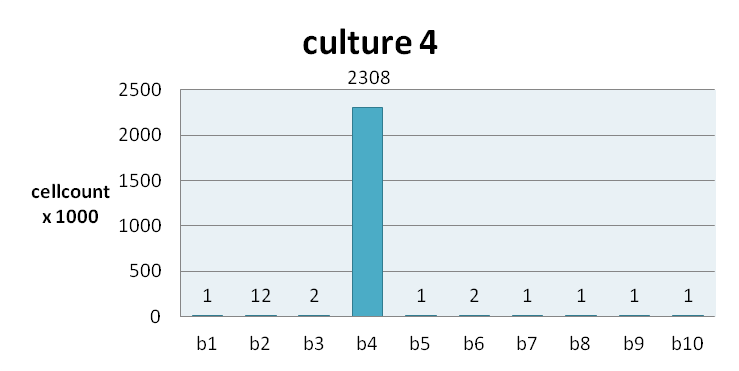
\includegraphics[scale = .2, trim = 5 5 5 5, clip]{c4.png} };
    \node[inner sep = 0 pt] (vdots) at (0, 2.5) {$\vdots$};
    \node[inner sep = 0 pt] (mid_evenness) at(0, 1.5)
    	{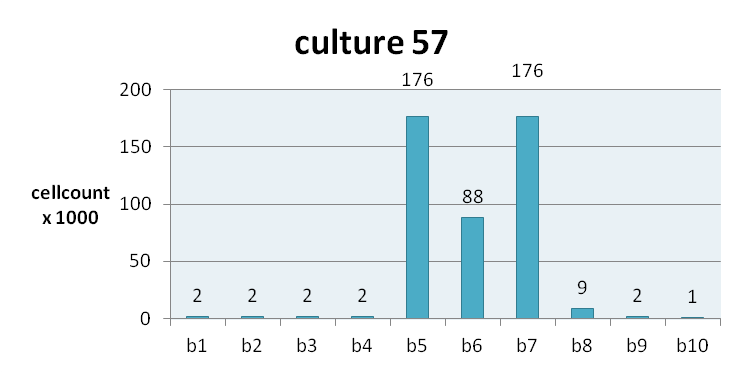
\includegraphics[scale = .2, trim = 5 5 5 5, clip]{c57.png}};
    \node[inner sep = 0 pt] (vdots) at (0, .5) {$\vdots$};
    \node[inner sep = 0 pt] (high_evenness) at(0, -.5)
       	{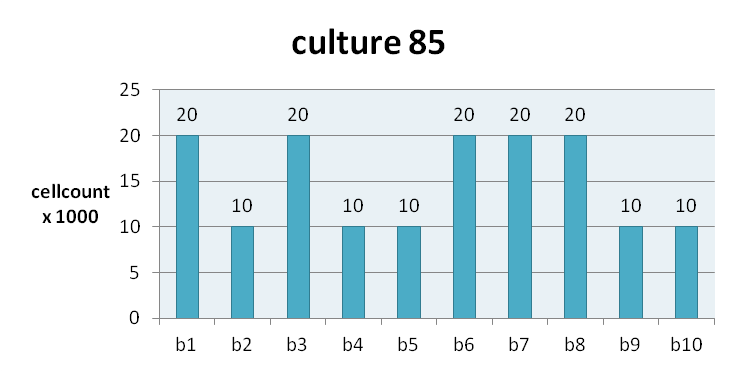
\includegraphics[scale = .2, trim = 5 5 5 5, clip]{c85.png}};
    \draw [decorate,decoration={brace,amplitude=10pt,mirror,raise=4pt},yshift=0pt]
    (1.5,-1) -- (1.5,3.6) node [black,midway,xshift=3.8cm] {   $\sim$ Pathogen behaviour after invasion};
	\end{tikzpicture}

\end{minipage} %\hfill
%\begin{minipage}{0.5\textwidth}
%Does evenness influence pathogen behaviour after invasion? 
%\end{minipage}
\end{frame}

\begin{frame}
\frametitle{Null hypothesis}
\begin{block}{Null hypothesis}
$
H_0: \mathcal{P(} \text{Invasion} \cap \text{evenness = High)} =\mathcal{P(} \text{Invasion} \cap \text{evenness = Low)}
$
\end{block}
\vspace*{.05in}
Ideally a 2-factor design tests for this hypothesis.

\begin{tikzpicture}
  \draw[->] (0,0) -- (7,0) node[right] {Pielou's evenness};
  \draw[->] (0,0) -- (0,3) node[above] {frequency};
  \draw[scale=0.5,domain=0:3,smooth,variable=\x,red] plot ({\x},{-\x*(\x-3)*2.5 });
  \draw[scale=0.5,domain=10:13,smooth,variable=\x,red] plot ({\x},{-(\x-10)*(\x-13)*2.5 });
\end{tikzpicture}

\end{frame}

\begin{frame}
\frametitle{Microbial aspect + Predictive aspect?}
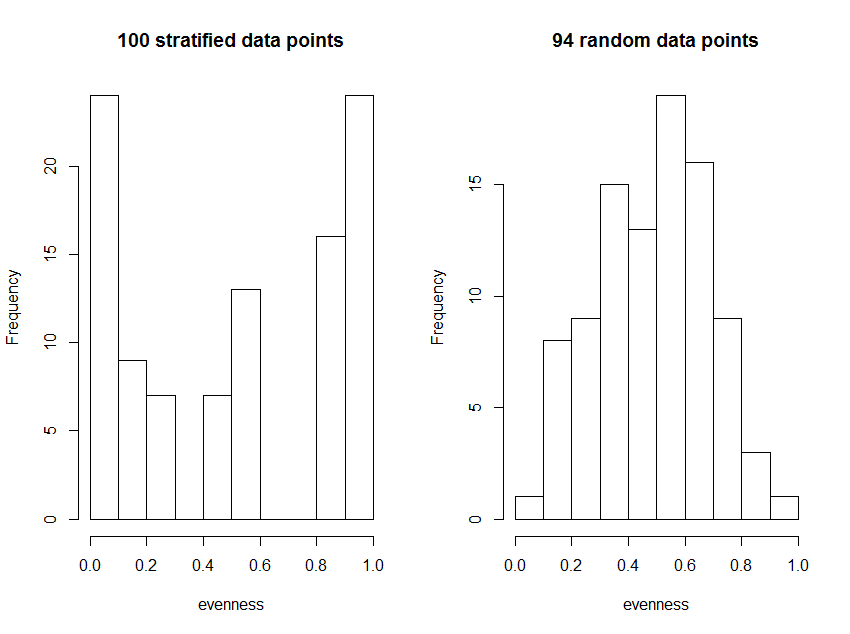
\includegraphics[scale = .3]{stratrandom.png};
\end{frame}

\begin{frame}
\frametitle{Final distribution}
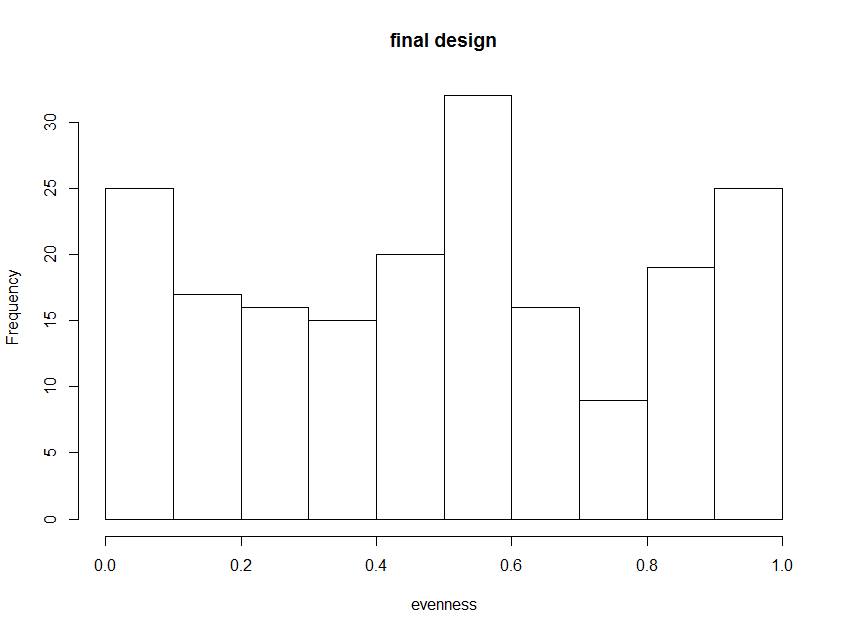
\includegraphics[scale = .3]{finalplot.png};
\end{frame}

%------------------------------------------------
\section{Material and Methods}
%------------------------------------------------

\begin{frame}
\frametitle{Selection Bacteria}

\begin{table}

\resizebox{0.8\textwidth}{!}{\begin{minipage}{\textwidth}
\centering
\begin{tabular}{l l l}

\toprule
\textbf{Bacteria} \\
\midrule
Pseudomonas sp. (10 TYP) \\
Bacillus sp. (1 Bacillus)  \\
Serratia sp. (14.3 ISO1) \\
Burkholderia Cepacia (Burkholderia) \\
Paracoccus sp. (42 Paracoccus)  \\
Enterococcus sp. (59 Enterococcus) \\
Agrobacterium sp. (Beijirinckia)  \\
Rhizobium Duejenense (63 Rhizobium)  \\
Delftia  \\
Aeromonas sp. (K62)  \\
\bottomrule
\end{tabular}
\caption{Selected Bacteria}
\end{minipage}}

\end{table}
\small{The bacteria are gathered from a waste water treatment plant. (cf. preliminary selection by Elham)}
\end{frame}

\begin{frame}
\frametitle{Which pathogen?}
\begin{itemize}
\item Investigate 5 - 10 pathogen from one phylogenetic family (Gammaproteobacteria)
\item Adjust number and selection after first results
\item Possibly follow-up with pathogen from different group
\end{itemize}

\end{frame}

%------------------------------------------------

\begin{frame}
\frametitle{Limiting conditions}
\begin{itemize}
\item Sample Throughput
\item Pipetting complexity
\item Quantifying the initial cell count
\end{itemize}
Solution: Preparing all cultures in advance and freezing them. 
\end{frame}

%------------------------------------------------

\begin{frame}
\frametitle{Preparing and freezing cultures}
% Make margins wider for this slide 
\Wider[4em]{

\begin{tikzpicture}
    \node[inner sep=0pt] (incubator) at (0,4.5)
    	{ \includegraphics[scale = .01, trim = 5 5 5 5, clip]{incubator.jpg} };
    \node[inner sep = 0 pt] (FCdilutions) at(0, 2.25)
    	{\includegraphics[scale = .01, trim = 5 5 5 5, clip]{FCdilutions.jpg}};
    \node[inner sep = 0 pt] (flowcytometer) at(0, 0)
    	{\includegraphics[scale = .01, trim = 5 5 5 5, clip]{flowcytometer.jpg}};
    \node[inner sep = 0 pt] (sampledilutions) at(6, 4.5)
       	{\includegraphics[scale = .01, trim = 5 5 5 5, clip]{sampledilutions.jpg}};
    \node[inner sep = 0 pt] (cryovials) at(6, 2.25)
       	{\includegraphics[scale = .01, trim = 5 5 5 5, clip]{cryovials.jpg}};
    \node (freezer) at (6, .5){freeze at -80 \degree C};       	
    % Draw some arrows
    %\draw[->] (0,0) -- (7,0) node[center] {FCdilutions};
	\draw[->,thick] (incubator.south) -- (FCdilutions.north)
    	node[midway,fill=white] {preparing dilutions};    
	\draw[->,thick] (FCdilutions.south) -- (flowcytometer.north)
    	node[midway,fill=white] {quantifying cell count};    	
    \draw [thick, ->](flowcytometer) .. controls ([yshift=-3cm, xshift=4cm] flowcytometer) and ([xshift=-3cm] sampledilutions) .. (sampledilutions)
    	node[midway,fill=white] {dilute sample};
	\draw[->,thick] (sampledilutions.south) -- (cryovials.north)
    	node[midway,fill=white] {pipet cultures};     
	\draw[->,thick] (sampledilutions.south) -- (cryovials.north)
    	node[midway,fill=white] {pipet cultures}; 	
	\draw[->,thick] (cryovials.south) -- (freezer.north);  	
	% Draw some accolades
    \draw [decorate,decoration={brace,amplitude=10pt,raise=4pt},yshift=0pt]
    (-1.5,-1) -- (-1.5,5.2) node [black,midway,xshift=-1.2cm] {8-13h};
    \draw [decorate,decoration={brace,amplitude=10pt, mirror,raise=4pt},yshift=0pt]
    (7.3,3.8) -- (7.3,5.2) node [black,midway,xshift=1.2cm] {13-14h};    
    \draw [decorate,decoration={brace,amplitude=10pt, mirror,raise=4pt},yshift=0pt]
    (7.3,0.2) -- (7.3,3) node [black,midway,xshift=1.2cm] {14-18h};        
\end{tikzpicture}

}
\end{frame}

\begin{frame}[fragile] % Need to use the fragile option when verbatim is used in the slide
\frametitle{Introducing pathogen}
\begin{enumerate}
\item Make the pathogens Streptomycin resistant
\item Introduce pathogen in each of the 194 cultures 
\item Plate in agar with Streptomycin 
\item Count colonies after 48h
\end{enumerate}
\end{frame}

%------------------------------------------------


%-------------------------------------
\section{Results}
%--------------------------------------

\begin{frame}
\frametitle{Progress so far?}
\begin{itemize}
\item 194 cultures prepared and in the freezer
\item A couple of pathogens made Streptomycin resistant
\item Start with first pathogen this week
\end{itemize}
\end{frame}


\begin{frame}
\frametitle{Conclusion}
\textbf{Optimistic Prognosis}
\begin{itemize}
\item Results of 5 to 10 pathogen mid November
\item First Predictive model before end of December
\end{itemize}
%\begin{figure}
%\includegraphics[width=0.8\linewidth]{test}
%\end{figure}
\end{frame}



%------------------------------------------------

\begin{frame}
\Huge{\centerline{The End}}
\end{frame}

%----------------------------------------------------------------------------------------

\end{document} 